% ViLexTime IEEE conference paper. Build: latexmk -xelatex main.tex
% Every number below traces to a file under runs/ or data/; see numbers.md next to this file.
\documentclass[conference]{IEEEtran}
\IEEEoverridecommandlockouts

\usepackage{newtxmath}
\usepackage[no-math]{fontspec}
\setmainfont{TeX Gyre Termes}
\usepackage{graphicx,booktabs,multirow,array,xcolor,pifont,makecell}
\usepackage{tikz,pgfplots}
\usetikzlibrary{positioning,arrows.meta,calc,fit,backgrounds,shapes.geometric,decorations.pathreplacing}
\pgfplotsset{compat=1.18}
\usepackage[hidelinks]{hyperref}
\usepackage[capitalise,nameinlink]{cleveref}
\usepackage{cite}

% palette (colour-blind safe, Okabe--Ito)
\definecolor{cBlue}{HTML}{0072B2}
\definecolor{cSky}{HTML}{56B4E9}
\definecolor{cOrange}{HTML}{E69F00}
\definecolor{cVerm}{HTML}{D55E00}
\definecolor{cGreen}{HTML}{009E73}
\definecolor{cGrey}{HTML}{7F7F7F}
\definecolor{cInk}{HTML}{1B2A41}

\newcommand{\cmark}{\textcolor{cGreen}{\ding{51}}}
\newcommand{\xmark}{\textcolor{cVerm}{\ding{55}}}
\newcommand{\sys}[1]{\textsf{#1}}
\newcommand{\vi}[1]{\textit{#1}}
\newcommand{\TBD}[1]{\textcolor{red}{[#1]}}

\begin{document}

\title{Right Law, Wrong Version: A Version-Aware Benchmark and a Controlled Analysis of Temporal Retrieval for Vietnamese Legal Question Answering}

\author{
\IEEEauthorblockN{Cao Minh Trí\IEEEauthorrefmark{1}, Nguyễn Minh Trí\IEEEauthorrefmark{1}, Đỗ Thị Minh Phụng\IEEEauthorrefmark{1}}
\IEEEauthorblockA{\IEEEauthorrefmark{1}University of Information Technology, Vietnam National University Ho Chi Minh City, Vietnam\\
Email: \{23521635, 23521643\}@gm.uit.edu.vn, \TBD{advisor email}}
}

\maketitle

\begin{abstract}
A legal question has an answer only at a point in time. Vietnamese statutes are frequently amended, partly repealed and restructured, so a retrieval-augmented generation (RAG) system can cite the right provision and still quote a wording that was not in force on the date the user asks about. We study this \emph{wrong-version} failure. First, we build a versioned corpus of 17{,}333 Vietnamese legal documents in which each provision keeps a stable identity and a history of wordings with half-open effective intervals, derived from amendment and repeal commands. Second, we release ViLexTime, a benchmark of question--date pairs whose gold answer is a specific provision version, scored contrastively: an answer must contain the span of the version in force and must not contain a span that only another version has. Third, under an analysis plan accepted before the final test set was run (156 provision lineages, 318 rows; two independent generation runs; Holm-corrected cluster bootstrap; confirmatory conditional on earlier pilot rounds), we compare a retrieval ladder that changes one component per step. Flat RAG quotes another version's text in 25--29\% of the rows where versions differ. Restricting candidates by document date and then by version interval raises version-exact Recall@1 by 7.8 and 11.5 points, and the full version-aware system improves accuracy over hybrid flat RAG by 34.3 points. Gold versions and filters share one derived store, labels are AI-produced with author review, and wrong-version rates are scorer-based. Post-hoc attribution suggests that the gain comes from the offline version store with hard interval filtering, that one-hop graph expansion at query time adds no detectable accuracy, and that most remaining errors occur when the in-force version is not ranked first.
\end{abstract}

\begin{IEEEkeywords}
legal question answering, temporal retrieval, retrieval-augmented generation, versioned corpora, Vietnamese law, benchmark
\end{IEEEkeywords}

% ======================================================================
\section{Introduction}
\label{sec:intro}

Statutory text is not static. Between two dates the same clause may receive a new wording, lose a point, be repealed through its parent article, or have its content moved to another document. A question such as \vi{``What is the maximum fine the Director of a Maritime Port Authority may impose?''} therefore has no single answer: in ViLexTime the gold answer is \vi{25{,}000{,}000 VND} for a question dated 16~February~2020 and \vi{50{,}000{,}000 VND} for the same question dated 19~July~2022 (\cref{fig:teaser}). A RAG system~\cite{lewis2020rag} that retrieves the topically best passage can return the right article and still answer with the wrong wording. We call this the \emph{wrong-version} error; it is distinct from retrieving an irrelevant passage and from refusing to answer.

Recent work shows that temporal filtering helps statutory question answering in German~\cite{prior2026oldfriend}, US federal regulations~\cite{yao2026lawinforce} and Thai law~\cite{akarajaradwong2026nitibenchplus}, and that both finding and applying the law in force are bottlenecks~\cite{yao2026lawinforce}. Graph-based RAG systems such as GraphRAG~\cite{edge2024graphrag} and LightRAG~\cite{guo2025lightrag} model relations between entities but not the validity of a wording on a date. Vietnamese legal QA resources~\cite{thanh2021alqac,nguyen2025vlqa,nguyen2026vihermes,dong2026vietlegal,nguyen2026vilegalexpert} are growing quickly, yet, in the sources we read, none grades an answer against the provision version in force at a user-supplied date. Two practical questions therefore remain open for Vietnamese law: how often do RAG systems answer with the wrong version, and which level of temporal information removes the error?

\begin{figure}[t]
\centering
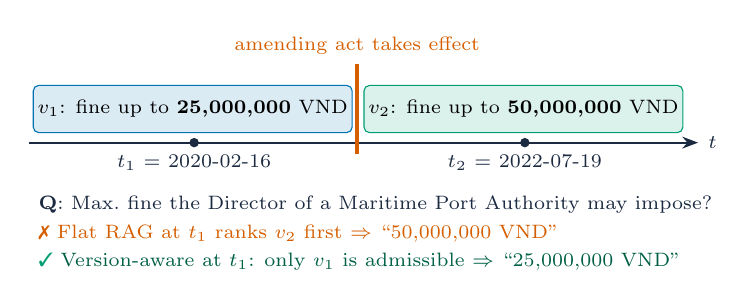
\begin{tikzpicture}[x=1cm,y=1cm,font=\scriptsize,
  ver/.style={draw=#1,fill=#1!14,rounded corners=2pt,minimum height=6mm,inner sep=1pt,align=center},
  lab/.style={font=\scriptsize,text=cInk}]
  \draw[-{Stealth[length=2mm]},cInk,thick] (0,0) -- (8.5,0) node[right,lab]{$t$};
  \node[ver=cBlue,anchor=south west,minimum width=4.05cm] (v1) at (0.05,0.12) {$v_1$: fine up to \textbf{25{,}000{,}000} VND};
  \node[ver=cGreen,anchor=south west,minimum width=4.05cm] (v2) at (4.25,0.12) {$v_2$: fine up to \textbf{50{,}000{,}000} VND};
  \draw[cVerm,very thick] (4.17,-0.15) -- (4.17,1.0);
  \node[lab,text=cVerm,anchor=south] at (4.17,1.0) {amending act takes effect};
  \foreach \x/\d/\n in {2.1/2020-02-16/1, 6.3/2022-07-19/2}{
     \fill[cInk] (\x,0) circle (1.7pt);
     \node[lab,below=1pt] at (\x,0) {$t_{\n}$ = \d};}
  \node[lab,anchor=north west] at (0.0,-0.55) {\textbf{Q}: Max.\ fine the Director of a Maritime Port Authority may impose?};
  \node[lab,anchor=north west,text=cVerm] at (0.0,-0.92) {\xmark\ Flat RAG at $t_1$ ranks $v_2$ first $\Rightarrow$ ``50{,}000{,}000 VND''};
  \node[lab,anchor=north west,text=cGreen!60!black] at (0.0,-1.28) {\cmark\ Version-aware at $t_1$: only $v_1$ is admissible $\Rightarrow$ ``25{,}000{,}000 VND''};
\end{tikzpicture}
\caption{The wrong-version error. One provision, two wordings with half-open effective intervals, and one question asked at two dates (an item of ViLexTime; text abridged and translated). The flat-RAG line is illustrative.}
\label{fig:teaser}
\end{figure}

We answer both questions with a resource and a controlled measurement. Our contributions are:
\begin{itemize}
\item \textbf{A versioned corpus of Vietnamese law} built from the official portal. Each provision has a stable identity, a chain of wordings derived by applying amendment and repeal commands, and effective intervals intersected with the intervals of its ancestors and its document (\cref{sec:corpus}).
\item \textbf{ViLexTime}, a benchmark of question--date pairs with version-level gold evidence, contrastive scoring that detects quoted text of a wrong version, and a full record of who or what produced each label; labels are AI-produced and author-reviewed, a silver tier (\cref{sec:benchmark}).
\item \textbf{A pre-specified evaluation on an unseen test set} of twelve generating configurations, including a retrieval ladder that adds one level of temporal information per step, two oracle conditions, two independent generation runs, and a human check of the scorer (\cref{sec:systems,sec:protocol,sec:results}).
\end{itemize}
The main findings are: flat RAG quotes another version in a quarter or more of the contrastive rows; giving the correct evidence lifts accuracy to 0.956, while giving the \emph{current} version instead drops it to 0.456; and both document-date filtering and version-interval filtering improve version-exact retrieval. Post-hoc attribution suggests that the benefit sits in the offline version store with hard interval filtering, while one-hop query-time graph expansion shows no measurable accuracy gain. Because gold versions and filters come from the same derived store, these results measure consistency with that store; \cref{sec:discussion} lists this and the other limits.

% ======================================================================
\section{Related Work}
\label{sec:related}

\textbf{Retrieval-augmented and graph-based generation.} RAG couples a retriever with a generator~\cite{lewis2020rag}; dense retrievers~\cite{karpukhin2020dpr} and BM25~\cite{robertson2009bm25} are combined in practice, e.g., by reciprocal rank fusion~\cite{cormack2009rrf}. GraphRAG builds an entity graph and community summaries for corpus-level questions~\cite{edge2024graphrag}; LightRAG retrieves over an LLM-extracted entity graph at two levels and expands one-hop neighbours~\cite{guo2025lightrag}. Statute retrieval has also used graph neural networks over the structure of codes~\cite{louis2023finding}. These graphs are entity- or structure-centric. Our graph is deterministic: nodes are provisions and versions, and edges are amendment and repeal events with dates.

\textbf{Time and versions.} TimeQA~\cite{chen2021timeqa} and TempLAMA~\cite{dhingra2022templama} pose the same question at several times for open-domain facts. VersionRAG models document versions for technical documentation~\cite{huwiler2025versionrag}. For law, de~Martim proposes an ontology-driven temporal graph of norms~\cite{demartim2025satgraph}; Prior et al.\ show that LLM consolidation of German amendments is error-prone~\cite{prior2025consolidation} and that a hard as-of filter strongly helps statutory QA~\cite{prior2026oldfriend}. LawShift evaluates judgment prediction under statute changes~\cite{han2025lawshift}. FiscalQA~Pro~\cite{cymbler2026fiscalqa} builds a versioned-corpus benchmark with deterministic scoring for French tax law; LawInForce-eCFR~\cite{yao2026lawinforce} and NitiBench+~\cite{akarajaradwong2026nitibenchplus} index dated versions and compare retrieval with and without temporal information. \Cref{tab:related} positions ViLexTime against them; its distinguishing feature is a ladder that separates document-date filtering, version-interval filtering and interval propagation on the same rows.

\textbf{Vietnamese legal QA.} ALQAC~\cite{thanh2021alqac} targets article retrieval and entailment; VLQA~\cite{nguyen2025vlqa}, VLegal-Bench~\cite{dong2026vietlegal} and ViLegalExpert~\cite{nguyen2026vilegalexpert} broaden scale and task coverage; ViHERMES studies multihop QA over healthcare regulations with a graph-aware retriever~\cite{nguyen2026vihermes}. None of the parts we read anchors the gold answer to a provision version at a question date.

\begin{table}[t]
\centering
\caption{Closest temporal legal QA benchmarks. \cmark: present; \xmark: absent; --: not determined from the sections we read.}
\label{tab:related}
\setlength{\tabcolsep}{2.4pt}
\scriptsize
\begin{tabular}{@{}l l c c c@{}}
\toprule
Benchmark & Jurisdiction & \makecell{Version gold\\at a date} & \makecell{Filter-level\\ladder} & \makecell{Repeal /\\no-answer} \\
\midrule
Prior et al.~\cite{prior2026oldfriend} & Germany & \cmark & \xmark & -- \\
FiscalQA Pro~\cite{cymbler2026fiscalqa} & France (tax) & \cmark & -- & -- \\
LawInForce-eCFR~\cite{yao2026lawinforce} & USA (federal) & \cmark & $\pm$date only & \xmark \\
NitiBench+~\cite{akarajaradwong2026nitibenchplus} & Thailand & \cmark & \xmark & \cmark \\
ViHERMES~\cite{nguyen2026vihermes} & Vietnam (health.) & -- & \xmark & -- \\
\midrule
\textbf{ViLexTime (ours)} & Vietnam & \cmark & \cmark\ (5 rungs) & \cmark \\
\bottomrule
\end{tabular}
\end{table}

% ======================================================================
\section{A Versioned Corpus of Vietnamese Law}
\label{sec:corpus}

\textbf{Representation.} We separate a provision's identity $p$ (an article, clause or point) from its wordings. A version $v$ of $p$ holds one wording valid over a local half-open interval $W_v=[s_v,e_v)$. A local interval is not enough: a clause whose parent article is repealed, or whose document has expired, is not in force even if its own wording was never touched. We therefore compute the effective interval offline as
\begin{equation}
\mathrm{Eff}(v) \;=\; W_v \,\cap\, C_{\mathrm{doc}(p)} \,\cap\! \bigcap_{a\in\mathrm{anc}(p)}\! C_a ,
\label{eq:eff}
\end{equation}
where $C_x$ is the union of the intervals in which node $x$ has a wording and $C_{\mathrm{doc}}$ is the validity of the owning document. Nodes that never carried text (e.g., a chapter heading) are transparent in the ancestor check. Disjoint pieces are kept, so a provision that lapses and is later re-enacted does not receive one covering interval. A unit $u$ is admissible at date $t$ when $t\in\mathrm{Eff}(u)$.

\textbf{From commands to versions.} Documents, structure trees and inter-document relations are crawled from the national legal database (vbpl.vn). An extractor recognises amending, supplementing, replacing and repealing commands together with structural locators (Article/Clause/Point), resolves their targets, and records operation type, effective date and source sentence. An event applier replays events on a copy of the provision state and commits a step only if the chain invariants still hold: an edit closes the open version at the event's effective date and opens a new one, and a repeal closes the target's chain. Events with ambiguous targets or missing text are queued for review instead of being guessed.

\textbf{Two retrieval layers.} Layer A contains the original wordings plus every amending or repealing command as a separate unit, so a flat baseline can still retrieve the sentence that wrote a new version. Layer B contains the materialised text of each version. \Cref{tab:corpus} gives the sizes.

\begin{table}[t]
\centering
\caption{Corpus used in all experiments (manifest counts) and quality checks of the version derivation.}
\label{tab:corpus}
\footnotesize
\begin{tabular}{@{}l r@{}}
\toprule
Documents owning corpus units & 17{,}333 \\
Layer A: original-wording units & 1{,}455{,}372 \\
Layer A: amending/repealing command units & 53{,}991 \\
Layer B: version units & 1{,}477{,}089 \\
\midrule
Earlier manual check of applied events$^\ast$ & 58/60 (96.7\%) \\
\quad Wilson 95\% interval & [88.6\%, 99.1\%] \\
Exact match with consolidated texts (51 docs) & 5{,}762/7{,}201 (80.0\%) \\
Expiry pairs covered by an applicable event & 3{,}238/8{,}046 (40.2\%) \\
\bottomrule
\multicolumn{2}{@{}p{0.95\columnwidth}@{}}{\scriptsize $^\ast$Historical sample, drawn before later extensions of the pipeline.}
\end{tabular}
\end{table}

The checks in \cref{tab:corpus} bound what the corpus can claim. Applied events were mostly correct in an earlier sample, but most expiry relations that the portal reports at document level have no applicable clause-level event yet: 5{,}200 of 8{,}046 pairs have an extracted event, only 3{,}238 an applicable one, and 1{,}109 have no event targeting the document at all. The consolidated texts used for comparison come from the same portal and are not an independent source.

% ======================================================================
\section{The ViLexTime Benchmark}
\label{sec:benchmark}

\textbf{Task.} Given a Vietnamese question $x$ and a date $t$, a system returns an answer $a$ and evidence $E$ at Article/Clause/Point level such that every $u\in E$ is admissible at $t$, or states that no provision in force answers the question. One row is one $(x,t)$ pair; rows sharing a provision lineage are dependent and are resampled together.

\begin{figure*}[t]
\centering
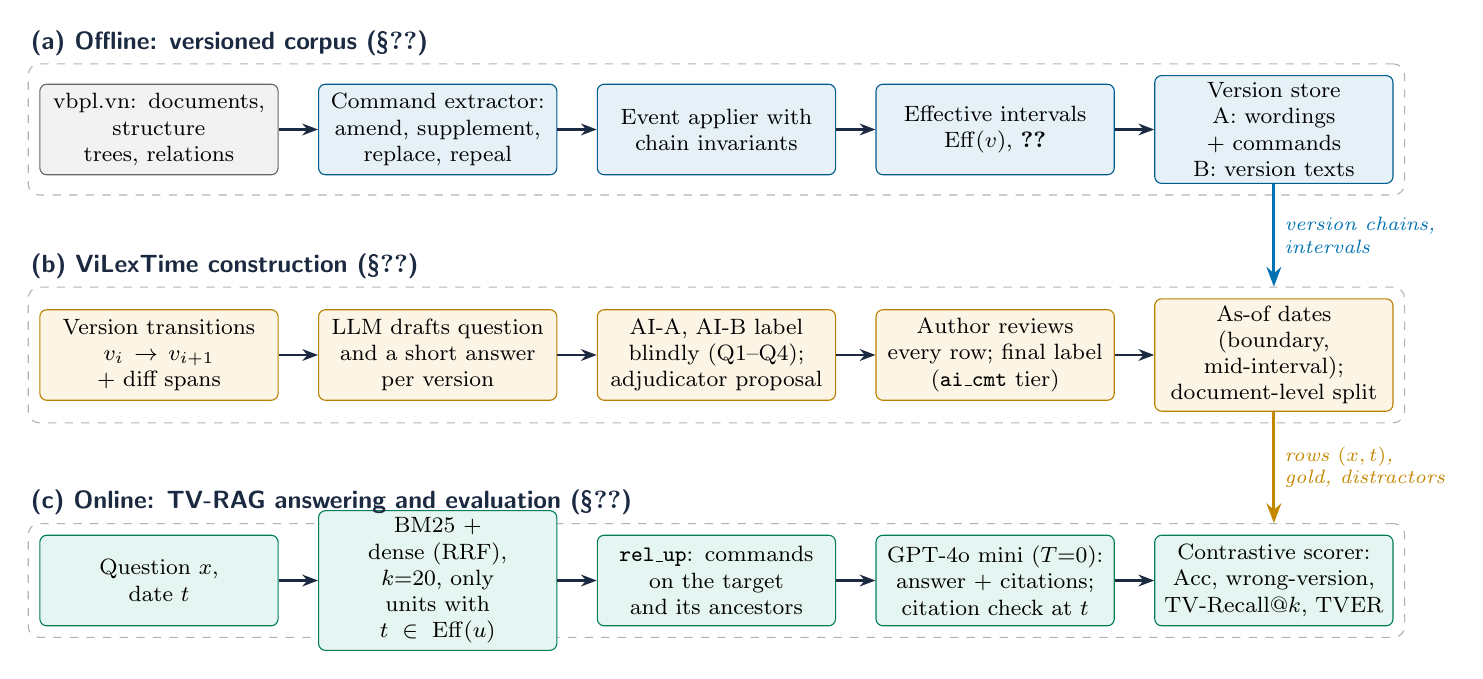
\begin{tikzpicture}[font=\footnotesize,node distance=3mm and 5mm,
  b/.style={draw=#1!80!black,fill=#1!10,rounded corners=2.5pt,align=center,inner sep=2.5pt,minimum height=11.5mm,text width=2.85cm},
  ar/.style={-{Stealth[length=2mm]},thick,cInk},
  panel/.style={draw=cGrey!60,dashed,rounded corners=4pt,inner sep=4pt},
  ptitle/.style={font=\small\bfseries\sffamily,text=cInk,anchor=south west,inner sep=1pt},
  flow/.style={-{Stealth[length=2.5mm]},line width=1.1pt}]
% (a)
\node[b=cGrey] (crawl) {vbpl.vn: documents,\\structure trees, relations};
\node[b=cBlue,right=of crawl] (ext) {Command extractor:\\amend, supplement,\\replace, repeal};
\node[b=cBlue,right=of ext] (app) {Event applier with\\chain invariants};
\node[b=cBlue,right=of app] (eff) {Effective intervals\\$\mathrm{Eff}(v)$, \cref{eq:eff}};
\node[b=cBlue,right=of eff] (store) {Version store\\A: wordings + commands\\B: version texts};
\foreach \u/\v in {crawl/ext,ext/app,app/eff,eff/store} \draw[ar] (\u) -- (\v);
% (b)
\node[b=cOrange,below=17mm of crawl] (cand) {Version transitions\\$v_i\!\to\!v_{i+1}$ + diff spans};
\node[b=cOrange,right=of cand] (q) {LLM drafts question\\and a short answer\\per version};
\node[b=cOrange,right=of q] (lab) {AI-A, AI-B label\\blindly (Q1--Q4);\\adjudicator proposal};
\node[b=cOrange,right=of lab] (rev) {Author reviews\\every row; final label\\(\texttt{ai\_cmt} tier)};
\node[b=cOrange,right=of rev] (asof) {As-of dates (boundary,\\mid-interval);\\document-level split};
\foreach \u/\v in {cand/q,q/lab,lab/rev,rev/asof} \draw[ar] (\u) -- (\v);
% (c)
\node[b=cGreen,below=17mm of cand] (query) {Question $x$,\\date $t$};
\node[b=cGreen,right=of query] (ret) {BM25 + dense (RRF),\\$k{=}20$, only units with\\$t\in\mathrm{Eff}(u)$};
\node[b=cGreen,right=of ret] (exp) {\texttt{rel\_up}: commands\\on the target\\and its ancestors};
\node[b=cGreen,right=of exp] (gen) {GPT-4o mini ($T{=}0$):\\answer + citations;\\citation check at $t$};
\node[b=cGreen,right=of gen] (score) {Contrastive scorer:\\Acc, wrong-version,\\TV-Recall@$k$, TVER};
\foreach \u/\v in {query/ret,ret/exp,exp/gen,gen/score} \draw[ar] (\u) -- (\v);
\begin{scope}[on background layer]
\node[panel,fit=(crawl)(store)] (P1) {};
\node[panel,fit=(cand)(asof)] (P2) {};
\node[panel,fit=(query)(score)] (P3) {};
\end{scope}
\node[ptitle] at ([yshift=0.6mm]P1.north west) {(a) Offline: versioned corpus (\S\ref{sec:corpus})};
\node[ptitle] at ([yshift=0.6mm]P2.north west) {(b) ViLexTime construction (\S\ref{sec:benchmark})};
\node[ptitle] at ([yshift=0.6mm]P3.north west) {(c) Online: TV-RAG answering and evaluation (\S\ref{sec:systems})};
\draw[flow,cBlue] (store.south) -- node[right,font=\scriptsize\itshape,text=cBlue,align=left]{version chains,\\intervals} (store.south |- P2.north);
\draw[flow,cOrange!85!black] (asof.south) -- node[right,font=\scriptsize\itshape,text=cOrange!85!black,align=left]{rows $(x,t)$,\\gold, distractors} (asof.south |- P3.north);
\end{tikzpicture}
\caption{Overview. (a) The version store is derived offline from amendment and repeal commands; effective intervals are precomputed. (b) Benchmark rows are generated from version transitions, labelled by two blind AI agents, and reviewed by an author. (c) At query time, retrieval reads layers A/B of the store and removes candidates outside their effective interval \emph{before} ranking; graph use at query time is limited to fetching commands that target the hit or its ancestors.}
\label{fig:overview}
\end{figure*}

\textbf{Construction.} \Cref{fig:overview}(b) summarises the pipeline. Candidates are version transitions of one provision with the spans that differ. An LLM drafts a question that is answerable from one provision and whose answer changes across the transition, together with a short answer span for each version. Rows are grouped by the phenomenon they probe: \textbf{T1} single-version provisions (controls), \textbf{T2} a pair of wordings before and after an amendment, \textbf{T3} chains of three or more versions, and \textbf{T6} provisions repealed directly or through a parent, whose correct answer after repeal is that no provision in force answers the question. A row whose content was moved to another document is excluded rather than labelled unanswerable, because a repeal at one location does not prove the content is gone.

\textbf{Dates and splits.} For each lineage we sample a \emph{boundary} date just after a transition and a \emph{mid-interval} date seeded away from both ends; main results use mid-interval dates, so the question date does not reveal which act just took effect. Dev and test are split by target document with a seeded hash, and the final test contains only lineages that no system had been run on.

\textbf{Labels and their provenance.} Every candidate row was labelled blindly and independently by two AI agents (AI-A, a Claude model; AI-B, a Codex model) against a four-question card: Q1 is each short answer correct for its date; Q2 does the question target the changed span; Q3 is the question unambiguous and non-leaking; Q4 does no other rule override the answer. A third agent proposed resolutions for disagreements and, under the first author's delegation, settled the hardest cases; the first author reviewed every row of the main slice and fixed the final label (the T1 control answers were not read by a human). Agreement between the two agents before reconciliation was Gwet's AC1~\cite{gwet2008ac1} = 0.608 on 314 lineages, below our 0.80 target. No lawyer or independent human labeller checked the final set. ViLexTime is therefore a documented silver resource with an explicit error record, not a legal gold standard; we report this tier with every result.

\begin{table}[t]
\centering
\caption{ViLexTime final test set (mid-interval rows). \textit{all} = T2+T3+T6 is the analysis slice; T1 is a control.}
\label{tab:data}
\footnotesize
\begin{tabular}{@{}l r r l@{}}
\toprule
Group & Lineages & Rows & Probes \\
\midrule
T2 & 127 & 254 & two wordings (76 rows near-identical) \\
T3 & 6 & 18 & chains of $\ge$3 versions \\
T6 & 23 & 46 & repeal (23 rows unanswerable) \\
\midrule
\textit{all} & 156 & 318 & 295 answerable \\
T1 (control) & 43 & 43 & single version \\
\bottomrule
\end{tabular}
\end{table}

\textbf{Scoring.} Accuracy is \emph{contrastive}: an answer is correct if it contains every gold span of the version in force at $t$ and none of the \emph{distractor} spans, i.e., spans that appear only in another version of the same provision; on unanswerable rows it is correct only if the system asserts that the provision is no longer in force (``I do not know'' is not a repeal claim). \emph{Wrong-version} is the share of rows with distractor spans whose answer contains one. TV-Recall@$k$ counts a hit only if the exact gold version (or accepted equivalent evidence) is in the top $k$; plain Recall@$k$ accepts any version of the provision. TVER is the share of answers with at least one resolved citation that cite at least one unit not admissible at $t$. Because TVER uses the same intervals as the filters, we treat it only as an internal consistency check.

% ======================================================================
\section{Systems}
\label{sec:systems}

All generating systems share one prompt, one generator (\texttt{gpt-4o-mini-2024-07-18}, temperature 0, 1{,}024 output tokens, fixed seed) and $k=20$. The prompt contains the question, the date and labelled evidence passages; the model must quote the wording valid at the date and cite labels, which are mapped back to unit identifiers. Dense retrieval uses \texttt{dangvantuan/vietnamese-embedding}; hybrid systems fuse BM25 and dense rankings by RRF ($k_{\mathrm{rrf}}=60$)~\cite{cormack2009rrf}; no system uses a reranker. \Cref{tab:systems} lists the configurations.

\begin{table}[t]
\centering
\caption{Compared configurations. Layer A: original wordings and commands; B: version texts. Filter: none, doc (document dates), ver (local version interval), prop (effective interval, \cref{eq:eff}).}
\label{tab:systems}
\setlength{\tabcolsep}{2.2pt}
\footnotesize
\begin{tabular}{@{}l l c c l l@{}}
\toprule
Name & ID & Layer & Filter & Retrieval & Query-time graph \\
\midrule
LLM only & \sys{b1} & -- & -- & none & -- \\
BM25 & \sys{b2ctx} & A & none & lexical & -- \\
Dense & \sys{b3} & A & none & dense & -- \\
Hybrid & \sys{b4} & A & none & hybrid & -- \\
Hybrid+AmendHop & \sys{b5} & A & none & hybrid & 1-hop commands \\
Hybrid+Hierarchy & \sys{b6} & A & none & hybrid & 1-hop parent/child \\
\midrule
+DocDate & \sys{b7} & A & doc & hybrid$^\dagger$ & -- \\
+VersionStore & \sys{b7v} & B & doc & lexical$^\dagger$ & -- \\
+VersionFilter & \sys{b7plus} & B & ver & hybrid$^\dagger$ & -- \\
+Propagation & \sys{b7pp} & B & prop & hybrid$^\dagger$ & -- \\
\textbf{TV-RAG} & \sys{proposed2} & B & prop & hybrid & \texttt{rel\_up} + check \\
\midrule
Oracle (in force) & \sys{oracle} & \multicolumn{4}{l}{in-force gold version is the only evidence} \\
Oracle (current) & \sys{oracle\_now} & \multicolumn{4}{l}{current version of the same provision} \\
\bottomrule
\multicolumn{6}{@{}p{0.97\columnwidth}@{}}{\scriptsize $^\dagger$The ladder tests F4--F6 use lexical retrieval for every rung; \sys{b7v} was run for retrieval only.}
\end{tabular}
\end{table}

\textbf{The ladder.} From \sys{b2ctx} to \sys{b7pp}, each rung changes one field: document-date filter (\sys{b7}), version texts instead of original wordings (\sys{b7v}), local version interval (\sys{b7plus}), and effective interval with ancestor propagation (\sys{b7pp}). Filters are applied inside the retrieval query, before the top-$k$ cut, not as post-filters on a short list.

\textbf{TV-RAG.} Our full system adds two query-time components to \sys{b7pp}. (i) \texttt{rel\_up} expansion takes the top seeds \emph{before} the date filter (after a repeal, the relevant provision may no longer be admissible) and adds commands that target the seed or any of its ancestors; commands are admitted by the validity of the document that issues them, and new units are appended after the ranked list (5 seeds, fan-out 3). (ii) A citation check rejects cited units not admissible at $t$; since the filter already removes such units, we expect it to act rarely and do not attribute gains to it. TV-RAG was selected on dev by a rule fixed in advance, before the final test was run.

\textbf{Graph baselines.} \sys{b5} and \sys{b6} are one-step expansions over amendment relations and the provision hierarchy inside the same pipeline. They are \emph{not} full GraphRAG or LightRAG systems; we name them accordingly.

% ======================================================================
\section{Evaluation Protocol}
\label{sec:protocol}

\textbf{Unseen test under a fixed plan.} The analysis plan (systems, metrics, slices, tests, decision rules and the selected system) was accepted and committed before the final test set was run. Two earlier rounds (a mixed human/agent-labelled set and an LLM-labelled replication, both with a 4B open model) and the dev set had been seen; we treat the final tests as confirmatory \emph{conditional} on that history and report it.

\textbf{Confirmatory family.} Seven paired tests, F1--F7 (\cref{tab:confirm}), are corrected with Holm's procedure~\cite{holm1979} at $\alpha=0.05$. Confidence intervals and $p$-values use a paired bootstrap with $B=10{,}000$ resamples of provision lineages, since rows of one lineage are dependent~\cite{dror2018hitchhiker}. F4--F6 are retrieval-only and deterministic. Because the generator is not deterministic at temperature 0, every generating system is run twice from identical prompts; a test is called \emph{supported} only if both runs agree. Run~1 is the pre-declared primary result. Anything outside F1--F7 is labelled \emph{descriptive} or \emph{exploratory (post hoc)}; exploratory numbers were computed after seeing the test results.

\textbf{Checking the scorer.} The first author scored 100 answers sampled with a fixed seed from run~1 (34 \sys{b1}, 33 \sys{b4}, 33 TV-RAG; T2/T3/T6), blind to system names and automatic scores, with no AI-drafted labels.

% ======================================================================
\section{Results}
\label{sec:results}

\subsection{How often does RAG use the wrong version? (descriptive)}

\Cref{fig:acc} reports accuracy on \textit{all}. Without retrieval, the generator almost never answers correctly (\sys{b1}: 0.006; the human scorer found 2/34 correct, mostly wrong content). Flat RAG answers about a third of the rows, and its answers contain a span that only another version has in 25.3\% (\sys{b2ctx}) and 29.1\% (\sys{b4}) of the rows with such spans (\cref{tab:main}). Non-temporal one-step graph expansion does not change this (\sys{b5}: 0.311; \sys{b6}: 0.340). The oracle pair isolates the temporal part of the problem: with the in-force version as the only evidence, the same generator reaches 0.956; with the current version of the same provision it reaches 0.456.

\begin{figure}[t]
\centering
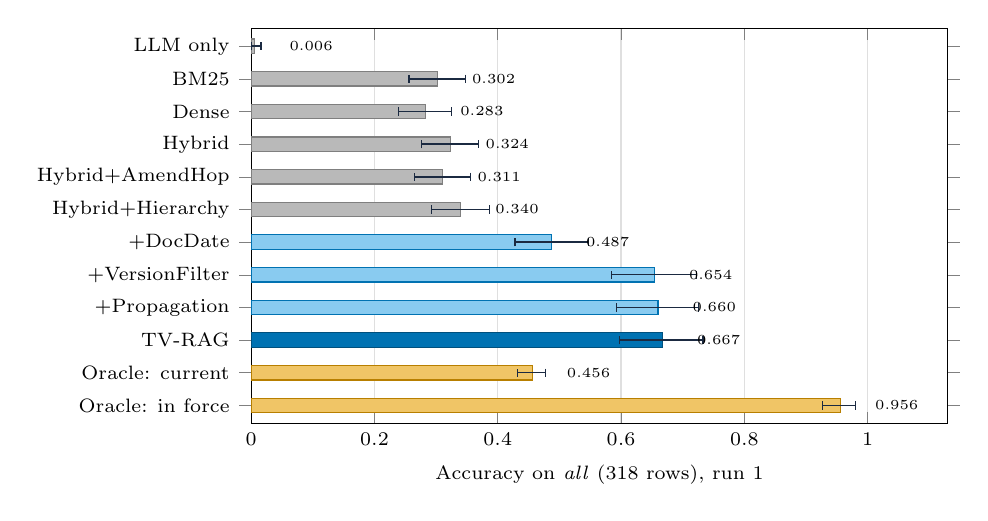
\begin{tikzpicture}
\begin{axis}[
  xbar, width=0.86\columnwidth, height=6.6cm,
  xmin=0, xmax=1.13, bar width=5.2pt,
  y dir=reverse, ytick={LLM only,BM25,Dense,Hybrid,Hybrid+AmendHop,Hybrid+Hierarchy,+DocDate,+VersionFilter,+Propagation,TV-RAG,Oracle: current,Oracle: in force}, enlarge y limits=0.05, bar shift=0pt,
  symbolic y coords={LLM only,BM25,Dense,Hybrid,Hybrid+AmendHop,Hybrid+Hierarchy,+DocDate,+VersionFilter,+Propagation,TV-RAG,Oracle: current,Oracle: in force},
  yticklabel style={font=\scriptsize}, xticklabel style={font=\scriptsize},
  xlabel={Accuracy on \textit{all} (318 rows), run 1}, xlabel style={font=\scriptsize},
  xmajorgrids, grid style={cGrey!25},
  nodes near coords, nodes near coords style={font=\tiny,anchor=west,xshift=9pt},
  point meta=explicit symbolic,
  error bars/x dir=both, error bars/x explicit, error bars/error bar style={cInk,line width=0.5pt}, error bars/error mark options={rotate=90,mark size=1.5pt},
]
\addplot[fill=cGrey!55,draw=cGrey] coordinates {
 (0.006,LLM only) += (0.010,0) -= (0.006,0) [0.006]
 (0.302,BM25) += (0.046,0) -= (0.046,0) [0.302]
 (0.283,Dense) += (0.042,0) -= (0.044,0) [0.283]
 (0.324,Hybrid) += (0.045,0) -= (0.047,0) [0.324]
 (0.311,Hybrid+AmendHop) += (0.045,0) -= (0.046,0) [0.311]
 (0.340,Hybrid+Hierarchy) += (0.046,0) -= (0.047,0) [0.340]};
\addplot[fill=cSky!70,draw=cBlue] coordinates {
 (0.487,+DocDate) += (0.060,0) -= (0.059,0) [0.487]
 (0.654,+VersionFilter) += (0.068,0) -= (0.069,0) [0.654]
 (0.660,+Propagation) += (0.066,0) -= (0.067,0) [0.660]};
\addplot[fill=cBlue,draw=cBlue!70!black] coordinates {(0.667,TV-RAG) += (0.066,0) -= (0.069,0) [0.667]};
\addplot[fill=cOrange!60,draw=cOrange!80!black] coordinates {
 (0.456,Oracle: current) += (0.022,0) -= (0.024,0) [0.456]
 (0.956,Oracle: in force) += (0.025,0) -= (0.029,0) [0.956]};
\end{axis}
\end{tikzpicture}
\caption{Accuracy with 95\% lineage-cluster bootstrap intervals. Grey: no temporal information; blue: temporal filters; orange: oracle evidence (same generator). Dense is \sys{b3}.}
\label{fig:acc}
\end{figure}

\begin{table}[t]
\centering
\caption{Descriptive results on \textit{all}, run 1 (318 rows). WV: wrong-version rate (lower is better; scorer-based). TV-R@1 here is over all 318 rows (unanswerable rows score 0) on the hybrid generation lists, unlike \cref{fig:ladder}.}
\label{tab:main}
\setlength{\tabcolsep}{3.5pt}
\footnotesize
\begin{tabular}{@{}l c c c c@{}}
\toprule
System & Accuracy [95\% CI] & TV-R@1 & TVER & WV \\
\midrule
LLM only & 0.006 [0.000, 0.016] & 0.000 & -- & 0.008 \\
BM25 & 0.302 [0.256, 0.348] & 0.151 & 0.535 & 0.253 \\
Hybrid & 0.324 [0.277, 0.369] & 0.164 & 0.544 & 0.291 \\
Hybrid+AmendHop & 0.311 [0.265, 0.356] & 0.164 & 0.566 & 0.294 \\
Hybrid+Hierarchy & 0.340 [0.293, 0.386] & 0.164 & 0.553 & 0.283 \\
+DocDate & 0.487 [0.428, 0.547] & 0.242 & 0.248 & 0.177 \\
+VersionFilter & 0.654 [0.585, 0.722] & 0.336 & 0.022 & 0.008 \\
+Propagation & 0.660 [0.593, 0.726] & 0.336 & 0.000 & 0.008 \\
\textbf{TV-RAG} & \textbf{0.667} [0.598, 0.733] & 0.336 & 0.013 & 0.008 \\
\midrule
Oracle (in force) & 0.956 [0.927, 0.981] & 1.000 & 0.000 & 0.000 \\
Oracle (current) & 0.456 [0.432, 0.478] & 0.484 & 0.516 & 0.502 \\
\bottomrule
\end{tabular}
\end{table}

\subsection{Confirmatory tests}

All six tests on the main slice are supported in both runs (\cref{tab:confirm}); because F6 coincides with F5 (below), they amount to five distinct findings. TV-RAG improves accuracy over hybrid flat RAG by 0.343 (F1) and over the non-temporal one-step graph baseline by 0.355 (F2), and lowers the wrong-version rate by 0.283 (F3). Document-date filtering (F4) and version-interval filtering (F5) both raise TV-Recall@1. F7, on the 23 unanswerable T6 rows, is inconclusive in both runs: with a minimum detectable effect of about 0.185 planned before the run, only very large effects were detectable, so this is not evidence of no effect.

\begin{table}[t]
\centering
\caption{Confirmatory family (Holm, $\alpha=0.05$; lineage-cluster bootstrap, $B=10{,}000$). P = TV-RAG. For F1--F6 no bootstrap resample reached the null in either run (Holm-adjusted $p<0.001$). $^\ast$Identical to F5; not evidence for propagation.}
\label{tab:confirm}
\setlength{\tabcolsep}{2.0pt}
\scriptsize
\begin{tabular}{@{}l l l c c@{}}
\toprule
 & Comparison (metric, slice) & Run 1 [95\% CI] & Run 2 & Verdict \\
\midrule
F1 & P$-$Hybrid (Acc, all) & $+$0.343 [$+$.283, $+$.401] & $+$0.368 & \cmark\ both \\
F2 & P$-$AmendHop (Acc, all) & $+$0.355 [$+$.297, $+$.414] & $+$0.352 & \cmark\ both \\
F3 & P$-$Hybrid (WV, all) & $-$0.283 [$-$.330, $-$.237] & $-$0.287 & \cmark\ both \\
F4 & DocDate$-$BM25 (TV-R@1, ans.) & $+$0.078 [$+$.049, $+$.110] & = & \cmark \\
F5 & VerFilter$-$DocDate (TV-R@1) & $+$0.115 [$+$.076, $+$.156] & = & \cmark \\
F6 & Propag.$-$DocDate (TV-R@1) & $+$0.115 [$+$.076, $+$.156] & = & \cmark$^\ast$ \\
F7 & P$-$Propag. (Acc, T6 unans.) & $+$0.087 [.000, $+$.217] & $+$0.043 & -- both \\
\bottomrule
\end{tabular}
\end{table}

F5 and F6 are numerically identical, and this matters for interpretation. \sys{b7pp} differs from \sys{b7plus} only by ancestor propagation; on the 295 answerable rows propagation changes the top-ranked unit in one row, where both are wrong. F6 is therefore supported entirely by the version-interval filter that F5 measures, and must not be read as evidence for propagation.

\subsection{Where does the gain come from? (post hoc)}

\Cref{fig:ladder} extends the ladder with \sys{b7v}, run for retrieval after the test was seen. Version texts \emph{without} interval filtering are worse than original wordings with a document filter ($-$0.044 [$-$0.072, $-$0.019]): a version store exposes every historical wording, so in this post-hoc, retrieval-only comparison it helps only when combined with the interval filter ($+$0.159 [$+$0.120, $+$0.199]).

\begin{figure}[t]
\centering
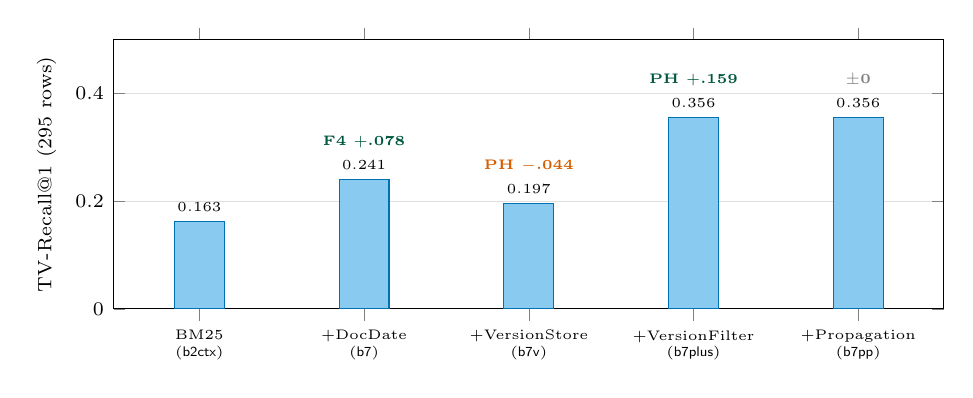
\begin{tikzpicture}
\begin{axis}[
  ybar, width=\columnwidth, height=5.0cm, bar width=18pt,
  ymin=0, ymax=0.5, ylabel={TV-Recall@1 (295 rows)}, ylabel style={font=\scriptsize},
  symbolic x coords={BM25,+DocDate,+VersionStore,+VersionFilter,+Propagation},
  xtick=data, xticklabels={BM25\\(\sys{b2ctx}),+DocDate\\(\sys{b7}),+VersionStore\\(\sys{b7v}),+VersionFilter\\(\sys{b7plus}),+Propagation\\(\sys{b7pp})},
  xticklabel style={font=\tiny,align=center},
  yticklabel style={font=\scriptsize}, ymajorgrids, grid style={cGrey!25},
  nodes near coords, nodes near coords style={font=\tiny}, enlarge x limits=0.13,
  every node near coord/.append style={/pgf/number format/fixed,/pgf/number format/precision=3},
]
\addplot[fill=cSky!70,draw=cBlue] coordinates {(BM25,0.1627) (+DocDate,0.2407) (+VersionStore,0.1966) (+VersionFilter,0.3559) (+Propagation,0.3559)};
\node[font=\tiny\bfseries,text=cGreen!55!black] at (axis cs:+DocDate,0.31) {F4 $+$.078};
\node[font=\tiny\bfseries,text=cVerm] at (axis cs:+VersionStore,0.265) {PH $-$.044};
\node[font=\tiny\bfseries,text=cGreen!55!black] at (axis cs:+VersionFilter,0.425) {PH $+$.159};
\node[font=\tiny\bfseries,text=cGrey] at (axis cs:+Propagation,0.425) {$\pm$0};
\end{axis}

\end{tikzpicture}
\caption{Retrieval ladder, lexical, $k=20$. Labels give the paired difference to the previous rung (F4: confirmatory; PH: post hoc). F5 = \textit{+VersionFilter} $-$ \textit{+DocDate} = $+$0.115.}
\label{fig:ladder}
\end{figure}

\textbf{Graph at query time.} On \textit{all}, TV-RAG minus \sys{b7plus} (same store and filter, no query-time graph) is $+$0.013 [$-$0.009, $+$0.035] in run~1 and $+$0.016 [$-$0.006, $+$0.038] in run~2; TV-RAG minus \sys{b7pp} is $+$0.006 and 0.000. The intervals contain zero in both runs, so we see no accuracy benefit larger than about four points from query-time graph use; we do not claim the systems are equal. On the 23 unanswerable T6 rows, TV-RAG beats \sys{b7plus} by $+$0.174 [$+$0.043, $+$0.348] in both runs, but half of that difference ($+$0.087) already separates \sys{b7pp} from \sys{b7plus}, and the test that isolates the query-time graph (F7) is inconclusive; a repeal benefit of the graph is therefore not established.

\textbf{Hard filtering versus telling the model the dates.} Two further baselines, added by a dated amendment to the plan after the test was seen and approved before they were run, read the version store with no filter (\sys{bvnone}) and with each passage's effective interval printed in the prompt (\sys{bvdate}). Printing dates raises accuracy from 0.311 to 0.409 and cuts the wrong-version rate from 0.317 to 0.064, but hard filtering before ranking is still far better: \sys{b7plus} minus \sys{bvdate} is $+$0.245 [$+$0.18, $+$0.31] in run~1 and $+$0.230 [$+$0.17, $+$0.29] in run~2.

\textbf{Repeal.} TV-RAG asserts that a provision is no longer in force 11 times, 7 correctly (precision 0.64, Wilson 95\% [0.35, 0.85]), recovering 7 of the 23 unanswerable rows (recall 0.30 [0.16, 0.51]). Flat BM25 also recovers 7 but makes 29 false repeal claims; the in-force oracle answers 22/23. Repeal detection remains weak for every retrieval system.

\subsection{Where the remaining errors occur (post hoc)}

\Cref{fig:rank} conditions TV-RAG's accuracy on the rank of the gold version in its prompt. When the gold version is ranked first, the answer is correct in 102 of 107 rows (95\%); accuracy falls with rank, to 8/20 at ranks 11--20 and 4/48 when the gold version is absent. The gold version is ranked first in only 107 of 295 answerable rows. Of the 247 rows whose prompt contains the gold version, 46 are still answered wrongly, 41 of them when the gold is below rank one. This is a correlational breakdown, not a causal test; it points to ranking within the admissible set, applied equally to all systems, as the most promising next step.

\begin{figure}[t]
\centering
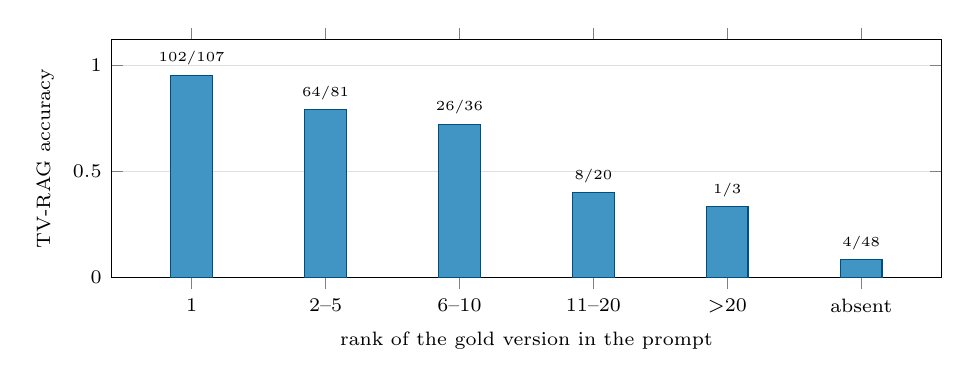
\begin{tikzpicture}
\begin{axis}[
  ybar, width=\columnwidth, height=4.6cm, bar width=15pt,
  ymin=0, ymax=1.12, ylabel={TV-RAG accuracy}, ylabel style={font=\scriptsize},
  symbolic x coords={1,2--5,6--10,11--20,$>$20,absent},
  xtick=data, xlabel={rank of the gold version in the prompt}, xlabel style={font=\scriptsize},
  xticklabel style={font=\scriptsize}, yticklabel style={font=\scriptsize},
  ymajorgrids, grid style={cGrey!25}, enlarge x limits=0.12,
  nodes near coords, point meta=explicit symbolic, nodes near coords style={font=\tiny,align=center},
]
\addplot[fill=cBlue!75,draw=cBlue!70!black] coordinates {
 (1,0.953) [102/107]
 (2--5,0.790) [64/81]
 (6--10,0.722) [26/36]
 (11--20,0.400) [8/20]
 ($>$20,0.333) [1/3]
 (absent,0.083) [4/48]};
\end{axis}
\end{tikzpicture}
\caption{TV-RAG accuracy (run 1, 295 answerable rows) by the rank of the gold version in the generation prompt. Labels: correct / rows.}
\label{fig:rank}
\end{figure}

\subsection{Is the scorer trustworthy?}

In a first, blind pass the automatic accuracy agreed with the human scorer on 95 of 100 answers ($\kappa=0.888$; Wilson 95\% [0.888, 0.979]); after one human label was revised (below), agreement is 96/100 ($\kappa=0.910$). In neither pass was an answer judged correct by the scorer but wrong by the human. In the four disagreements the human accepted the answer: three paraphrase the gold span or use a different enumeration mark, and one contains the gold span together with a span of another version. The revision was made after seeing the disagreements and an AI assistant's suggestion to re-check three items. A single scorer, who is also an author, judged all 100 answers. The human counts per system (\sys{b1} 2/34, \sys{b4} 10/33, TV-RAG 23/33) follow the same order as F1. We therefore use no LLM judge for accuracy. The sheet showed only the in-force version, so it could not validate the wrong-version flag; F3 and all wrong-version rates are scorer-based.

\textbf{Subset with blind human gold.} For 24 of the 156 lineages (53 rows; no T6) a human built the gold version blind to the graph; it matched the graph-derived gold on 119 of 120 items after AI-proposed, author-confirmed adjudication. Scored with the release labels, F1--F6 point in the same direction on this subset in both runs (e.g., F5 $+$0.189 [$+$0.071, $+$0.315]). This is descriptive and does not replace independent gold for the whole set.

% ======================================================================
\section{Discussion and Limitations}
\label{sec:discussion}

\textbf{What the results support.} For Vietnamese law, the large and robust effect is that of \emph{knowing which wording is in force}: an offline version store plus a hard interval filter before ranking. This agrees with the as-of filtering results for German, US and Thai law~\cite{prior2026oldfriend,yao2026lawinforce,akarajaradwong2026nitibenchplus}; what ViLexTime adds is a decomposition on the same rows, whose post-hoc steps suggest that a version store without the filter hurts and that printing dates in the prompt does not substitute for filtering. The graph's main role is offline, in deriving versions and intervals; at query time we detect no gain, and a repeal-specific benefit is not established.

\textbf{Threats to validity.} (i) \emph{Shared source.} Gold versions and filter intervals come from the same derived graph; when an event is missed, both can be wrong together, so F3--F6 measure consistency with the graph. Blind gold covers only 24/156 lineages and no T6. (ii) \emph{Labels.} The final set is AI-labelled and reviewed by the first author, with pre-reconciliation AI--AI AC1 of 0.608 and hard cases settled by an AI adjudicator under author delegation; no lawyer checked them. (iii) \emph{Coverage.} T3 (6 lineages) and T6 (23) are small, 76 of the 254 T2 rows are near-identical wordings, T5 (retroactive or signed-but-not-yet-effective) is absent, and 220 of the 318 rows fall outside the four target domains. The T1 short answers were found, after the run, to contain whole clause text with enumeration marks, making the T1 column unusable; it is excluded and will be corrected only through a declared amendment. (iv) \emph{Scope.} One generator, no reranker and one source portal; \sys{b5}/\sys{b6} are one-step expansions, not full GraphRAG, and a LightRAG comparison is pending. (v) \emph{Selection.} The confirmatory family was fixed after the dev set and two pilot rounds had been seen.

% ======================================================================
\section{Conclusion}
\label{sec:conclusion}

We presented a versioned corpus of Vietnamese law, the ViLexTime benchmark with contrastive version-level scoring, and a pre-specified one-shot evaluation. Flat RAG frequently quotes the wrong version. Measured against the derived store, temporal filtering removes most of those scorer-detected errors, and post-hoc attribution places the benefit in the offline version store with hard interval filtering rather than in query-time graph traversal. The next steps are independent human gold and lawyer checks of the final set, higher clause-level event coverage, better ranking among admissible units, and a second generator family. Code, data and run artefacts with hashes are released with the paper.

% ======================================================================
\section*{Statements and Declarations}
\footnotesize
\textbf{Data availability.} ViLexTime (release files, metadata, manifest and SHA-256 sums), the corpus derivation code, the analysis plans and all run artefacts behind every number are available at \url{https://github.com/cmtri2005/graphrag-legal-thesis}. Source texts are public legal documents from vbpl.vn. \textbf{Ethics.} The study uses public legal texts and involves no personal data or human subjects beyond the authors. ViLexTime is a research benchmark and must not be used as legal advice. \textbf{Author contributions (CRediT).} \TBD{to be completed by the authors: conceptualization, data curation, software, investigation, validation, writing, supervision}. \textbf{Competing interests.} The authors declare none. \textbf{Funding.} \TBD{state funding or ``none''}. \textbf{Use of AI.} AI agents (Claude and Codex models) drafted benchmark questions, produced the two blind label sets and adjudication proposals described in \cref{sec:benchmark}, and assisted with code and with drafting this manuscript; GPT-4o mini is the evaluated generator. The first author reviewed all final labels of the main slice and produced the human scoring of 100 answers without AI-drafted labels; the authors take full responsibility for all claims.

\bibliographystyle{IEEEtran}
\bibliography{references}

\end{document}
